\documentclass{report} 
\title{Strang}
\date{Started 5th June 2025}
\author{Malcolm}
\usepackage{amsmath} %import math
\usepackage{mathtools} %more math
\usepackage{amssymb} %for QED symbol
\usepackage{amsthm} %
\usepackage{bm}%bold math
\usepackage{graphicx} %import imaging
\graphicspath{{./images/}} %set imaging path
\begin{document}
\maketitle

\tableofcontents

\newpage

\chapter{Vectors and Matrices}
\section{Intuition for Dot product, Cosine formula, Schwarz and Triangle inequalities}
\textbf{Intuition for dot product}\\
The unit vectors $\bm{v}=(\cos\alpha,\sin\alpha)$ and $\bm{w}=(\cos\beta,\sin\beta)$ are plotted as follows
\begin{center}
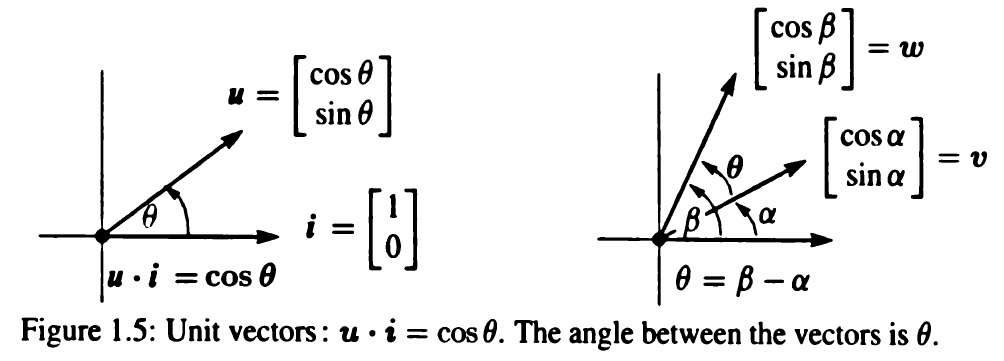
\includegraphics[width=10cm]{1}
\end{center}
See first that when fixed in this form, the magnitude of both vectors is 1, with an angle $\beta-\alpha$ between them. These unit vectors have dot product
\begin{equation*}
\bm{v}\cdot\bm{w}=\cos\alpha\cos\beta+\sin\alpha\sin\beta=\cos(\beta-\alpha)
\end{equation*}
We have $\theta$ as the angle between the two vectors; see that the sign of $\bm v\cdot\bm w$ tells us whether $\theta$ is below or above a right angle (due
to the cosine function being negative for its argument $>\pi/2$ and positive for $<\pi/2$):
\begin{center}
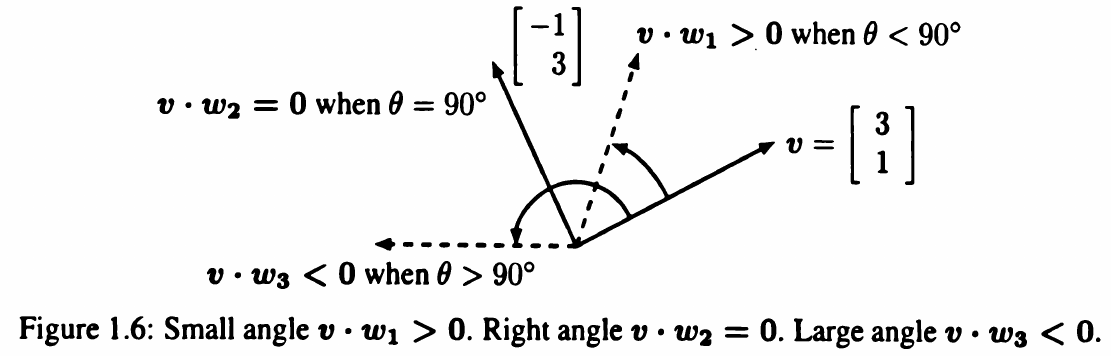
\includegraphics[width=9cm]{2}
\end{center}
(next page)\newpage
\noindent\textbf{Cont.}\\
The idea here is that the dot product reveals the exact angle $\theta$; for unit vectors $\bm u$ and $\bm U$, the dot product $\bm u\cdot\bm U$ is the cosine of 
$\theta$. Ths remains true in $n$ dimensions (not shown).\\
\vspace{1mm}\\
See that any $\bm{u}$ and $\bm{v}$ can be fixed in the above form by normalising their lengths to get
$\bm u=\bm v/||\bm v||$ and $\bm U=\bm w/||\bm w||$. After which their dot product would give $\cos\theta$. This leads us to the \textit{cosine formula}:
\begin{equation*}
\text{\textbf{Cosine formula}: }
\frac{\bm v\cdot\bm w}{||\bm v||\,||\bm w||}=\cos\theta\quad\text{ if $\bm v$ and $\bm w$ are nonzero vectors}
\end{equation*}
\textbf{Perpendicular vectors}\\
See that when the angle between $\bm v$ and $\bm w$ is $90^\circ$, its cosine is 0; this gives us a way to test this. Also see that for perpendicular vectors:
\begin{equation*}
||\bm v+\bm w||^2=||\bm v||^2+||\bm w||^2
\end{equation*}
because
\begin{equation*}
||\bm v+\bm w||^2=(\bm v+\bm w)\cdot(\bm v+\bm w)=\bm v\cdot\bm v+\bm v\cdot\bm w+\bm w\cdot\bm v+\bm w\cdot\bm w
\end{equation*}
where $\bm v\cdot \bm w=0$.\\
\vspace{1mm}\\
\textbf{Schwarz and Triangle inequalities}\\
First, see from the cosine formula that the dot product of $\bm v/||\bm v||$ and
$\bm w/||\bm w||$ never exceeds one (since $\cos\theta$ never exceeds one). This is the the 
\textit{Schwarz inequality}:
\begin{equation*}
\text{\textbf{Schwarz inequality}: }|\bm v\cdot\bm w|\leq||\bm v||\,||\bm w||
\end{equation*}
The \textit{Triangle inequality} comes directly from the Schwarz inequality:
\begin{equation*}
\text{\textbf{Triangle inequality}: }||\bm v+\bm w||\leq||\bm v||+||\bm w||
\end{equation*}
This can be seen from
\begin{equation*}
||\bm v+\bm w||^2=\bm v\cdot\bm v+\bm v\cdot\bm w+\bm w\cdot\bm v+\bm w\cdot\bm w
\leq||\bm v||^2+2||\bm v||\,||\bm w||+||\bm w||^2
\end{equation*}
The square root gives us the triangle equality (side 3 cannot exceed side 1 + side 2).
\newpage

\section{}







\end{document}
